\subsection{CU18 Eliminar Refacción}
Esta pantalla funciona como un mensaje de seguridad, este se asegurará que el administrador realmente quiere eliminar el registro que ha seleccionado de una refacción, mostrará toda la información que se tiene sobre esa refacción. En la parte inferior hay dos botones:
\begin{itemize}
	\item \textbf{Aceptar:} El sistema elimina el registro seleccionado por el administrador y muestra un mensaje de confirmación que el proceso ha sido exitoso.
	\item \textbf{Cancelar:} El sistema regresa a la pantalla anterior (figura \ref{fig:Pantalla Visualizar Refacciones Administrador - Vista de Escenarios}) sin hacer alguna modificación.
\end{itemize}
{\begin{figure}[!h]
	\centering
	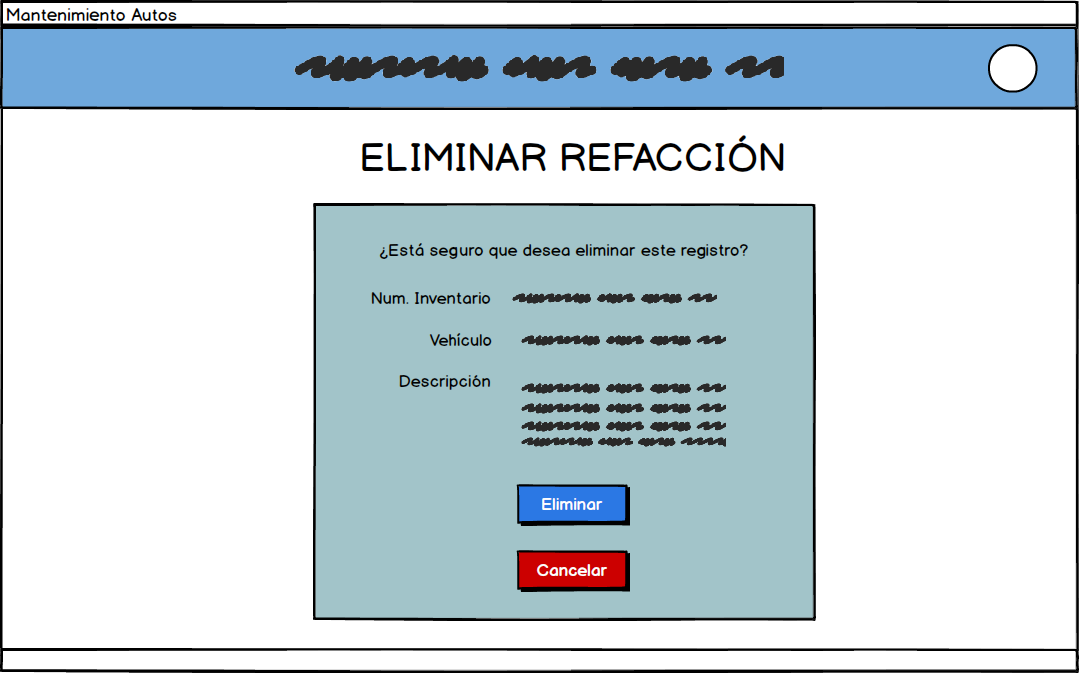
\includegraphics[width=0.8\textwidth]{./diseno/vescenarios/imagenes/eliminarRefaccion}
	\caption{Pantalla Eliminar Refacciones  - Vista de Escenarios}
	\label{fig:Pantalla Eliminar Refacción - Vista de Escenarios}
\end{figure}
\begin{figure}[!h]
	\centering
	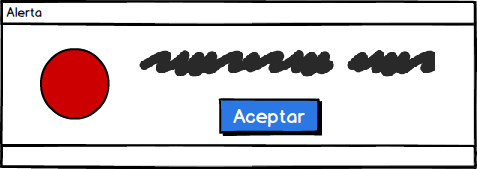
\includegraphics[width=0.3\textwidth]{./diseno/vescenarios/imagenes/alerta}
	\caption{Alerta Eliminar Refacciones- Vista de Escenarios}
	\label{fig:Alerta Eliminar Refacciones - Vista de Escenarios}
\end{figure}
\clearpage